\documentclass[1p]{elsarticle_modified}
%\bibliographystyle{elsarticle-num}

%\usepackage[colorlinks]{hyperref}
%\usepackage{abbrmath_seonhwa} %\Abb, \Ascr, \Acal ,\Abf, \Afrak
\usepackage{amsfonts}
\usepackage{amssymb}
\usepackage{amsmath}
\usepackage{amsthm}
\usepackage{scalefnt}
\usepackage{amsbsy}
\usepackage{kotex}
\usepackage{caption}
\usepackage{subfig}
\usepackage{color}
\usepackage{graphicx}
\usepackage{xcolor} %% white, black, red, green, blue, cyan, magenta, yellow
\usepackage{float}
\usepackage{setspace}
\usepackage{hyperref}

\usepackage{tikz}
\usetikzlibrary{arrows}

\usepackage{multirow}
\usepackage{array} % fixed length table
\usepackage{hhline}

%%%%%%%%%%%%%%%%%%%%%
\makeatletter
\renewcommand*\env@matrix[1][\arraystretch]{%
	\edef\arraystretch{#1}%
	\hskip -\arraycolsep
	\let\@ifnextchar\new@ifnextchar
	\array{*\c@MaxMatrixCols c}}
\makeatother %https://tex.stackexchange.com/questions/14071/how-can-i-increase-the-line-spacing-in-a-matrix
%%%%%%%%%%%%%%%

\usepackage[normalem]{ulem}

\newcommand{\msout}[1]{\ifmmode\text{\sout{\ensuremath{#1}}}\else\sout{#1}\fi}
%SOURCE: \msout is \stkout macro in https://tex.stackexchange.com/questions/20609/strikeout-in-math-mode

\newcommand{\cancel}[1]{
	\ifmmode
	{\color{red}\msout{#1}}
	\else
	{\color{red}\sout{#1}}
	\fi
}

\newcommand{\add}[1]{
	{\color{blue}\uwave{#1}}
}

\newcommand{\replace}[2]{
	\ifmmode
	{\color{red}\msout{#1}}{\color{blue}\uwave{#2}}
	\else
	{\color{red}\sout{#1}}{\color{blue}\uwave{#2}}
	\fi
}

\newcommand{\Sol}{\mathcal{S}} %segment
\newcommand{\D}{D} %diagram
\newcommand{\A}{\mathcal{A}} %arc


%%%%%%%%%%%%%%%%%%%%%%%%%%%%%5 test

\def\sl{\operatorname{\textup{SL}}(2,\Cbb)}
\def\psl{\operatorname{\textup{PSL}}(2,\Cbb)}
\def\quan{\mkern 1mu \triangleright \mkern 1mu}

\theoremstyle{definition}
\newtheorem{thm}{Theorem}[section]
\newtheorem{prop}[thm]{Proposition}
\newtheorem{lem}[thm]{Lemma}
\newtheorem{ques}[thm]{Question}
\newtheorem{cor}[thm]{Corollary}
\newtheorem{defn}[thm]{Definition}
\newtheorem{exam}[thm]{Example}
\newtheorem{rmk}[thm]{Remark}
\newtheorem{alg}[thm]{Algorithm}

\newcommand{\I}{\sqrt{-1}}
\begin{document}

%\begin{frontmatter}
%
%\title{Boundary parabolic representations of knots up to 8 crossings}
%
%%% Group authors per affiliation:
%\author{Yunhi Cho} 
%\address{Department of Mathematics, University of Seoul, Seoul, Korea}
%\ead{yhcho@uos.ac.kr}
%
%
%\author{Seonhwa Kim} %\fnref{s_kim}}
%\address{Center for Geometry and Physics, Institute for Basic Science, Pohang, 37673, Korea}
%\ead{ryeona17@ibs.re.kr}
%
%\author{Hyuk Kim}
%\address{Department of Mathematical Sciences, Seoul National University, Seoul 08826, Korea}
%\ead{hyukkim@snu.ac.kr}
%
%\author{Seokbeom Yoon}
%\address{Department of Mathematical Sciences, Seoul National University, Seoul, 08826,  Korea}
%\ead{sbyoon15@snu.ac.kr}
%
%\begin{abstract}
%We find all boundary parabolic representation of knots up to 8 crossings.
%
%\end{abstract}
%\begin{keyword}
%    \MSC[2010] 57M25 
%\end{keyword}
%
%\end{frontmatter}

%\linenumbers
%\tableofcontents
%
\newcommand\colored[1]{\textcolor{white}{\rule[-0.35ex]{0.8em}{1.4ex}}\kern-0.8em\color{red} #1}%
%\newcommand\colored[1]{\textcolor{white}{ #1}\kern-2.17ex	\textcolor{white}{ #1}\kern-1.81ex	\textcolor{white}{ #1}\kern-2.15ex\color{red}#1	}

{\Large $\underline{12a_{0864}~(K12a_{0864})}$}

\setlength{\tabcolsep}{10pt}
\renewcommand{\arraystretch}{1.6}
\vspace{1cm}\begin{tabular}{m{100pt}>{\centering\arraybackslash}m{274pt}}
\multirow{5}{120pt}{
	\centering
	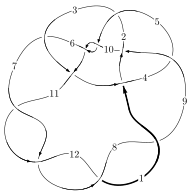
\includegraphics[width=112pt]{../../../GIT/diagram.site/Diagrams/png/1665_12a_0864.png}\\
\ \ \ A knot diagram\footnotemark}&
\allowdisplaybreaks
\textbf{Linearized knot diagam} \\
\cline{2-2}
 &
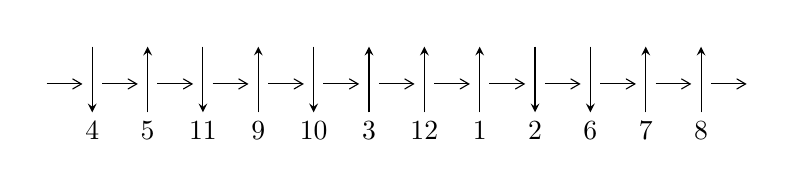
\begin{tikzpicture}[x=20pt, y=17pt]
	% nodes
	\node (C0) at (0, 0) {};
	\node (C1) at (1, 0) {};
	\node (C1U) at (1, +1) {};
	\node (C1D) at (1, -1) {4};

	\node (C2) at (2, 0) {};
	\node (C2U) at (2, +1) {};
	\node (C2D) at (2, -1) {5};

	\node (C3) at (3, 0) {};
	\node (C3U) at (3, +1) {};
	\node (C3D) at (3, -1) {11};

	\node (C4) at (4, 0) {};
	\node (C4U) at (4, +1) {};
	\node (C4D) at (4, -1) {9};

	\node (C5) at (5, 0) {};
	\node (C5U) at (5, +1) {};
	\node (C5D) at (5, -1) {10};

	\node (C6) at (6, 0) {};
	\node (C6U) at (6, +1) {};
	\node (C6D) at (6, -1) {3};

	\node (C7) at (7, 0) {};
	\node (C7U) at (7, +1) {};
	\node (C7D) at (7, -1) {12};

	\node (C8) at (8, 0) {};
	\node (C8U) at (8, +1) {};
	\node (C8D) at (8, -1) {1};

	\node (C9) at (9, 0) {};
	\node (C9U) at (9, +1) {};
	\node (C9D) at (9, -1) {2};

	\node (C10) at (10, 0) {};
	\node (C10U) at (10, +1) {};
	\node (C10D) at (10, -1) {6};

	\node (C11) at (11, 0) {};
	\node (C11U) at (11, +1) {};
	\node (C11D) at (11, -1) {7};

	\node (C12) at (12, 0) {};
	\node (C12U) at (12, +1) {};
	\node (C12D) at (12, -1) {8};
	\node (C13) at (13, 0) {};

	% arrows
	\draw[->,>={angle 60}]
	(C0) edge (C1) (C1) edge (C2) (C2) edge (C3) (C3) edge (C4) (C4) edge (C5) (C5) edge (C6) (C6) edge (C7) (C7) edge (C8) (C8) edge (C9) (C9) edge (C10) (C10) edge (C11) (C11) edge (C12) (C12) edge (C13) ;	\draw[->,>=stealth]
	(C1U) edge (C1D) (C2D) edge (C2U) (C3U) edge (C3D) (C4D) edge (C4U) (C5U) edge (C5D) (C6D) edge (C6U) (C7D) edge (C7U) (C8D) edge (C8U) (C9U) edge (C9D) (C10U) edge (C10D) (C11D) edge (C11U) (C12D) edge (C12U) ;
	\end{tikzpicture} \\
\hhline{~~} \\& 
\textbf{Solving Sequence} \\ \cline{2-2} 
 &
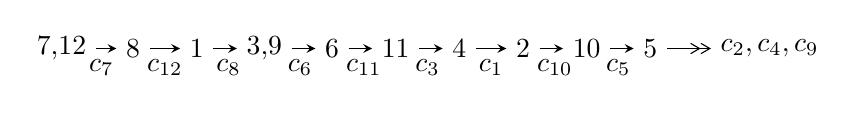
\begin{tikzpicture}[x=23pt, y=7pt]
	% node
	\node (A0) at (-1/8, 0) {7,12};
	\node (A1) at (1, 0) {8};
	\node (A2) at (2, 0) {1};
	\node (A3) at (49/16, 0) {3,9};
	\node (A4) at (33/8, 0) {6};
	\node (A5) at (41/8, 0) {11};
	\node (A6) at (49/8, 0) {4};
	\node (A7) at (57/8, 0) {2};
	\node (A8) at (65/8, 0) {10};
	\node (A9) at (73/8, 0) {5};
	\node (C1) at (1/2, -1) {$c_{7}$};
	\node (C2) at (3/2, -1) {$c_{12}$};
	\node (C3) at (5/2, -1) {$c_{8}$};
	\node (C4) at (29/8, -1) {$c_{6}$};
	\node (C5) at (37/8, -1) {$c_{11}$};
	\node (C6) at (45/8, -1) {$c_{3}$};
	\node (C7) at (53/8, -1) {$c_{1}$};
	\node (C8) at (61/8, -1) {$c_{10}$};
	\node (C9) at (69/8, -1) {$c_{5}$};
	\node (A10) at (11, 0) {$c_{2},c_{4},c_{9}$};

	% edge
	\draw[->,>=stealth]	
	(A0) edge (A1) (A1) edge (A2) (A2) edge (A3) (A3) edge (A4) (A4) edge (A5) (A5) edge (A6) (A6) edge (A7) (A7) edge (A8) (A8) edge (A9) ;
	\draw[->>,>={angle 60}]	
	(A9) edge (A10);
\end{tikzpicture} \\ 

\end{tabular} \\

\footnotetext{
The image of knot diagram is generated by the software ``\textbf{Draw programme}" developed by Andrew Bartholomew(\url{http://www.layer8.co.uk/maths/draw/index.htm\#Running-draw}), where we modified some parts for our purpose(\url{https://github.com/CATsTAILs/LinksPainter}).
}\phantom \\ \newline 
\centering \textbf{Ideals for irreducible components\footnotemark of $X_{\text{par}}$} 
 
\begin{align*}
I^u_{1}&=\langle 
-1.21264\times10^{139} u^{95}+1.73441\times10^{139} u^{94}+\cdots+1.05860\times10^{139} b+1.91553\times10^{139},\\
\phantom{I^u_{1}}&\phantom{= \langle  }-3.04022\times10^{140} u^{95}+1.79659\times10^{139} u^{94}+\cdots+1.05860\times10^{139} a+2.01484\times10^{141},\\
\phantom{I^u_{1}}&\phantom{= \langle  }u^{96}-61 u^{94}+\cdots-28 u-1\rangle \\
I^u_{2}&=\langle 
u^{15}- u^{14}+\cdots+b+2,\;- u^{15}+2 u^{14}+\cdots+a-9,\;u^{16}-12 u^{14}+\cdots+5 u+1\rangle \\
I^u_{3}&=\langle 
b-1,\;a+2,\;u+1\rangle \\
\\
\end{align*}
\raggedright * 3 irreducible components of $\dim_{\mathbb{C}}=0$, with total 113 representations.\\
\footnotetext{All coefficients of polynomials are rational numbers. But the coefficients are sometimes approximated in decimal forms when there is not enough margin.}
\newpage
\renewcommand{\arraystretch}{1}
\centering \section*{I. $I^u_{1}= \langle -1.21\times10^{139} u^{95}+1.73\times10^{139} u^{94}+\cdots+1.06\times10^{139} b+1.92\times10^{139},\;-3.04\times10^{140} u^{95}+1.80\times10^{139} u^{94}+\cdots+1.06\times10^{139} a+2.01\times10^{141},\;u^{96}-61 u^{94}+\cdots-28 u-1 \rangle$}
\flushleft \textbf{(i) Arc colorings}\\
\begin{tabular}{m{7pt} m{180pt} m{7pt} m{180pt} }
\flushright $a_{7}=$&$\begin{pmatrix}1\\0\end{pmatrix}$ \\
\flushright $a_{12}=$&$\begin{pmatrix}0\\u\end{pmatrix}$ \\
\flushright $a_{8}=$&$\begin{pmatrix}1\\- u^2\end{pmatrix}$ \\
\flushright $a_{1}=$&$\begin{pmatrix}u\\- u^3+u\end{pmatrix}$ \\
\flushright $a_{3}=$&$\begin{pmatrix}28.7194 u^{95}-1.69714 u^{94}+\cdots-3987.96 u-190.331\\1.14552 u^{95}-1.63841 u^{94}+\cdots-76.6899 u-1.80950\end{pmatrix}$ \\
\flushright $a_{9}=$&$\begin{pmatrix}- u^2+1\\u^4-2 u^2\end{pmatrix}$ \\
\flushright $a_{6}=$&$\begin{pmatrix}18.9381 u^{95}-4.14300 u^{94}+\cdots-1887.37 u-59.3130\\2.76827 u^{95}-0.450564 u^{94}+\cdots-370.656 u-18.2747\end{pmatrix}$ \\
\flushright $a_{11}=$&$\begin{pmatrix}- u\\u\end{pmatrix}$ \\
\flushright $a_{4}=$&$\begin{pmatrix}26.6420 u^{95}-4.78463 u^{94}+\cdots-3924.43 u-186.996\\3.22295 u^{95}+1.44908 u^{94}+\cdots-140.220 u-5.14505\end{pmatrix}$ \\
\flushright $a_{2}=$&$\begin{pmatrix}-3.95609 u^{95}-0.462103 u^{94}+\cdots+390.837 u+0.542360\\3.87936 u^{95}+0.714479 u^{94}+\cdots-343.306 u-13.3366\end{pmatrix}$ \\
\flushright $a_{10}=$&$\begin{pmatrix}-4.26382 u^{95}+1.69030 u^{94}+\cdots-9.12211 u-30.4716\\-3.77515 u^{95}+0.646135 u^{94}+\cdots+455.415 u+22.4214\end{pmatrix}$ \\
\flushright $a_{5}=$&$\begin{pmatrix}31.0772 u^{95}-2.97999 u^{94}+\cdots-4218.61 u-199.407\\1.95541 u^{95}-1.75880 u^{94}+\cdots-157.514 u-5.53567\end{pmatrix}$\\&\end{tabular}
\flushleft \textbf{(ii) Obstruction class $= -1$}\\~\\
\flushleft \textbf{(iii) Cusp Shapes $= -3.53643 u^{95}+0.820615 u^{94}+\cdots+864.770 u+50.5047$}\\~\\
\newpage\renewcommand{\arraystretch}{1}
\flushleft \textbf{(iv) u-Polynomials at the component}\newline \\
\begin{tabular}{m{50pt}|m{274pt}}
Crossings & \hspace{64pt}u-Polynomials at each crossing \\
\hline $$\begin{aligned}c_{1}\end{aligned}$$&$\begin{aligned}
&u^{96}+5 u^{95}+\cdots-4478 u+638
\end{aligned}$\\
\hline $$\begin{aligned}c_{2}\end{aligned}$$&$\begin{aligned}
&u^{96}-8 u^{95}+\cdots+5 u-1
\end{aligned}$\\
\hline $$\begin{aligned}c_{3}\end{aligned}$$&$\begin{aligned}
&u^{96}+5 u^{94}+\cdots-723 u-97
\end{aligned}$\\
\hline $$\begin{aligned}c_{4}\end{aligned}$$&$\begin{aligned}
&u^{96}+2 u^{95}+\cdots-5914 u-463
\end{aligned}$\\
\hline $$\begin{aligned}c_{5},c_{10}\end{aligned}$$&$\begin{aligned}
&u^{96}-2 u^{95}+\cdots+4 u+2
\end{aligned}$\\
\hline $$\begin{aligned}c_{6}\end{aligned}$$&$\begin{aligned}
&u^{96}-9 u^{94}+\cdots-872 u-79
\end{aligned}$\\
\hline $$\begin{aligned}c_{7},c_{8},c_{11}\\c_{12}\end{aligned}$$&$\begin{aligned}
&u^{96}-61 u^{94}+\cdots+28 u-1
\end{aligned}$\\
\hline $$\begin{aligned}c_{9}\end{aligned}$$&$\begin{aligned}
&u^{96}-3 u^{95}+\cdots-1819 u+211
\end{aligned}$\\
\hline
\end{tabular}\\~\\
\newpage\renewcommand{\arraystretch}{1}
\flushleft \textbf{(v) Riley Polynomials at the component}\newline \\
\begin{tabular}{m{50pt}|m{274pt}}
Crossings & \hspace{64pt}Riley Polynomials at each crossing \\
\hline $$\begin{aligned}c_{1}\end{aligned}$$&$\begin{aligned}
&y^{96}+23 y^{95}+\cdots-5697484 y+407044
\end{aligned}$\\
\hline $$\begin{aligned}c_{2}\end{aligned}$$&$\begin{aligned}
&y^{96}+6 y^{95}+\cdots-947 y+1
\end{aligned}$\\
\hline $$\begin{aligned}c_{3}\end{aligned}$$&$\begin{aligned}
&y^{96}+10 y^{95}+\cdots+487817 y+9409
\end{aligned}$\\
\hline $$\begin{aligned}c_{4}\end{aligned}$$&$\begin{aligned}
&y^{96}-32 y^{95}+\cdots-43540896 y+214369
\end{aligned}$\\
\hline $$\begin{aligned}c_{5},c_{10}\end{aligned}$$&$\begin{aligned}
&y^{96}-74 y^{95}+\cdots+592 y+4
\end{aligned}$\\
\hline $$\begin{aligned}c_{6}\end{aligned}$$&$\begin{aligned}
&y^{96}-18 y^{95}+\cdots-426056 y+6241
\end{aligned}$\\
\hline $$\begin{aligned}c_{7},c_{8},c_{11}\\c_{12}\end{aligned}$$&$\begin{aligned}
&y^{96}-122 y^{95}+\cdots-208 y+1
\end{aligned}$\\
\hline $$\begin{aligned}c_{9}\end{aligned}$$&$\begin{aligned}
&y^{96}-29 y^{95}+\cdots-3023067 y+44521
\end{aligned}$\\
\hline
\end{tabular}\\~\\
\newpage\flushleft \textbf{(vi) Complex Volumes and Cusp Shapes}
$$\begin{array}{c|c|c}  
\text{Solutions to }I^u_{1}& \I (\text{vol} + \sqrt{-1}CS) & \text{Cusp shape}\\
 \hline 
\begin{aligned}
u &= \phantom{-}0.848856 + 0.512394 I \\
a &= -1.48444 + 0.02987 I \\
b &= \phantom{-}1.13304 + 1.13103 I\end{aligned}
 & \phantom{-}1.79803 + 6.02425 I & \phantom{-0.000000 } 0 \\ \hline\begin{aligned}
u &= \phantom{-}0.848856 - 0.512394 I \\
a &= -1.48444 - 0.02987 I \\
b &= \phantom{-}1.13304 - 1.13103 I\end{aligned}
 & \phantom{-}1.79803 - 6.02425 I & \phantom{-0.000000 } 0 \\ \hline\begin{aligned}
u &= -0.762783 + 0.552893 I \\
a &= \phantom{-}0.084512 - 0.657058 I \\
b &= \phantom{-}0.480853 + 0.094565 I\end{aligned}
 & \phantom{-}1.63897 - 1.62411 I & \phantom{-0.000000 } 0 \\ \hline\begin{aligned}
u &= -0.762783 - 0.552893 I \\
a &= \phantom{-}0.084512 + 0.657058 I \\
b &= \phantom{-}0.480853 - 0.094565 I\end{aligned}
 & \phantom{-}1.63897 + 1.62411 I & \phantom{-0.000000 } 0 \\ \hline\begin{aligned}
u &= -0.872654 + 0.313471 I \\
a &= \phantom{-}1.57203 + 0.70936 I \\
b &= -0.771400 + 0.941898 I\end{aligned}
 & -2.26631 - 4.65369 I & \phantom{-0.000000 } 0 \\ \hline\begin{aligned}
u &= -0.872654 - 0.313471 I \\
a &= \phantom{-}1.57203 - 0.70936 I \\
b &= -0.771400 - 0.941898 I\end{aligned}
 & -2.26631 + 4.65369 I & \phantom{-0.000000 } 0 \\ \hline\begin{aligned}
u &= \phantom{-}0.943151 + 0.542936 I \\
a &= \phantom{-}1.046870 - 0.578677 I \\
b &= -0.950136 - 0.507528 I\end{aligned}
 & \phantom{-}4.03768 + 8.33548 I & \phantom{-0.000000 } 0 \\ \hline\begin{aligned}
u &= \phantom{-}0.943151 - 0.542936 I \\
a &= \phantom{-}1.046870 + 0.578677 I \\
b &= -0.950136 + 0.507528 I\end{aligned}
 & \phantom{-}4.03768 - 8.33548 I & \phantom{-0.000000 } 0 \\ \hline\begin{aligned}
u &= \phantom{-}0.910484\phantom{ +0.000000I} \\
a &= -0.878663\phantom{ +0.000000I} \\
b &= -0.378648\phantom{ +0.000000I}\end{aligned}
 & -3.16205\phantom{ +0.000000I} & \phantom{-0.000000 } 0 \\ \hline\begin{aligned}
u &= \phantom{-}0.811946 + 0.726956 I \\
a &= \phantom{-}0.149340 + 0.747403 I \\
b &= \phantom{-}0.505940 - 0.747645 I\end{aligned}
 & -2.10344 - 4.68024 I & \phantom{-0.000000 } 0\\
 \hline 
 \end{array}$$\newpage$$\begin{array}{c|c|c}  
\text{Solutions to }I^u_{1}& \I (\text{vol} + \sqrt{-1}CS) & \text{Cusp shape}\\
 \hline 
\begin{aligned}
u &= \phantom{-}0.811946 - 0.726956 I \\
a &= \phantom{-}0.149340 - 0.747403 I \\
b &= \phantom{-}0.505940 + 0.747645 I\end{aligned}
 & -2.10344 + 4.68024 I & \phantom{-0.000000 } 0 \\ \hline\begin{aligned}
u &= -0.951904 + 0.531798 I \\
a &= -1.65073 - 0.27863 I \\
b &= \phantom{-}1.17052 - 1.03295 I\end{aligned}
 & -1.00269 - 14.05450 I & \phantom{-0.000000 } 0 \\ \hline\begin{aligned}
u &= -0.951904 - 0.531798 I \\
a &= -1.65073 + 0.27863 I \\
b &= \phantom{-}1.17052 + 1.03295 I\end{aligned}
 & -1.00269 + 14.05450 I & \phantom{-0.000000 } 0 \\ \hline\begin{aligned}
u &= -0.849730 + 0.148988 I \\
a &= \phantom{-}1.28832 - 0.69583 I \\
b &= -0.310227 + 0.149527 I\end{aligned}
 & \phantom{-}1.94088 - 0.58707 I & \phantom{-0.000000 } 0 \\ \hline\begin{aligned}
u &= -0.849730 - 0.148988 I \\
a &= \phantom{-}1.28832 + 0.69583 I \\
b &= -0.310227 - 0.149527 I\end{aligned}
 & \phantom{-}1.94088 + 0.58707 I & \phantom{-0.000000 } 0 \\ \hline\begin{aligned}
u &= -0.066590 + 0.860109 I \\
a &= \phantom{-}0.044443 + 0.190892 I \\
b &= -0.667589 + 0.223840 I\end{aligned}
 & \phantom{-}0.94601 - 3.74110 I & \phantom{-0.000000 } 0 \\ \hline\begin{aligned}
u &= -0.066590 - 0.860109 I \\
a &= \phantom{-}0.044443 - 0.190892 I \\
b &= -0.667589 - 0.223840 I\end{aligned}
 & \phantom{-}0.94601 + 3.74110 I & \phantom{-0.000000 } 0 \\ \hline\begin{aligned}
u &= \phantom{-}0.851105 + 0.131792 I \\
a &= \phantom{-}1.01100 + 2.07444 I \\
b &= -0.236581 - 0.169350 I\end{aligned}
 & \phantom{-}0.90358 + 5.68147 I & \phantom{-0.000000 } 0 \\ \hline\begin{aligned}
u &= \phantom{-}0.851105 - 0.131792 I \\
a &= \phantom{-}1.01100 - 2.07444 I \\
b &= -0.236581 + 0.169350 I\end{aligned}
 & \phantom{-}0.90358 - 5.68147 I & \phantom{-0.000000 } 0 \\ \hline\begin{aligned}
u &= \phantom{-}0.847214 + 0.071086 I \\
a &= -1.54881 + 0.33064 I \\
b &= \phantom{-}1.119980 + 0.555179 I\end{aligned}
 & \phantom{-}4.24776 + 1.77300 I & \phantom{-0.000000 } 0\\
 \hline 
 \end{array}$$\newpage$$\begin{array}{c|c|c}  
\text{Solutions to }I^u_{1}& \I (\text{vol} + \sqrt{-1}CS) & \text{Cusp shape}\\
 \hline 
\begin{aligned}
u &= \phantom{-}0.847214 - 0.071086 I \\
a &= -1.54881 - 0.33064 I \\
b &= \phantom{-}1.119980 - 0.555179 I\end{aligned}
 & \phantom{-}4.24776 - 1.77300 I & \phantom{-0.000000 } 0 \\ \hline\begin{aligned}
u &= \phantom{-}1.15263\phantom{ +0.000000I} \\
a &= -2.79307\phantom{ +0.000000I} \\
b &= \phantom{-}1.59079\phantom{ +0.000000I}\end{aligned}
 & \phantom{-}1.49561\phantom{ +0.000000I} & \phantom{-0.000000 } 0 \\ \hline\begin{aligned}
u &= -1.012410 + 0.563472 I \\
a &= \phantom{-}0.915243 + 0.270713 I \\
b &= -0.830878 + 0.373538 I\end{aligned}
 & \phantom{-}3.91381 - 1.35031 I & \phantom{-0.000000 } 0 \\ \hline\begin{aligned}
u &= -1.012410 - 0.563472 I \\
a &= \phantom{-}0.915243 - 0.270713 I \\
b &= -0.830878 - 0.373538 I\end{aligned}
 & \phantom{-}3.91381 + 1.35031 I & \phantom{-0.000000 } 0 \\ \hline\begin{aligned}
u &= \phantom{-}0.776553 + 0.310353 I \\
a &= -0.378054 + 0.041126 I \\
b &= \phantom{-}0.132735 + 0.970644 I\end{aligned}
 & \phantom{-}1.05313 + 4.13427 I & \phantom{-0.000000 } 0 \\ \hline\begin{aligned}
u &= \phantom{-}0.776553 - 0.310353 I \\
a &= -0.378054 - 0.041126 I \\
b &= \phantom{-}0.132735 - 0.970644 I\end{aligned}
 & \phantom{-}1.05313 - 4.13427 I & \phantom{-0.000000 } 0 \\ \hline\begin{aligned}
u &= -1.140350 + 0.241058 I \\
a &= \phantom{-}0.287971 + 0.490780 I \\
b &= -0.752610 - 0.354976 I\end{aligned}
 & -0.561295 + 0.360803 I & \phantom{-0.000000 } 0 \\ \hline\begin{aligned}
u &= -1.140350 - 0.241058 I \\
a &= \phantom{-}0.287971 - 0.490780 I \\
b &= -0.752610 + 0.354976 I\end{aligned}
 & -0.561295 - 0.360803 I & \phantom{-0.000000 } 0 \\ \hline\begin{aligned}
u &= \phantom{-}0.094602 + 0.804581 I \\
a &= -0.126983 + 0.252363 I \\
b &= \phantom{-}0.872343 + 0.988761 I\end{aligned}
 & -4.18034 + 9.61860 I & \phantom{-0.000000 } 0 \\ \hline\begin{aligned}
u &= \phantom{-}0.094602 - 0.804581 I \\
a &= -0.126983 - 0.252363 I \\
b &= \phantom{-}0.872343 - 0.988761 I\end{aligned}
 & -4.18034 - 9.61860 I & \phantom{-0.000000 } 0\\
 \hline 
 \end{array}$$\newpage$$\begin{array}{c|c|c}  
\text{Solutions to }I^u_{1}& \I (\text{vol} + \sqrt{-1}CS) & \text{Cusp shape}\\
 \hline 
\begin{aligned}
u &= -0.793794 + 0.085736 I \\
a &= \phantom{-}1.86729 - 0.01780 I \\
b &= -1.14389 + 1.32461 I\end{aligned}
 & \phantom{-}0.16910 - 5.24105 I & \phantom{-0.000000 } 0 \\ \hline\begin{aligned}
u &= -0.793794 - 0.085736 I \\
a &= \phantom{-}1.86729 + 0.01780 I \\
b &= -1.14389 - 1.32461 I\end{aligned}
 & \phantom{-}0.16910 + 5.24105 I & \phantom{-0.000000 } 0 \\ \hline\begin{aligned}
u &= \phantom{-}0.695579 + 0.387592 I \\
a &= \phantom{-}1.59202 - 1.13315 I \\
b &= -0.963161 - 0.805203 I\end{aligned}
 & -3.16653 + 6.53955 I & \phantom{-0.000000 } 0 \\ \hline\begin{aligned}
u &= \phantom{-}0.695579 - 0.387592 I \\
a &= \phantom{-}1.59202 + 1.13315 I \\
b &= -0.963161 + 0.805203 I\end{aligned}
 & -3.16653 - 6.53955 I & \phantom{-0.000000 } 0 \\ \hline\begin{aligned}
u &= -0.737621 + 0.059931 I \\
a &= -2.65688 + 1.12940 I \\
b &= \phantom{-}0.868841 + 0.104292 I\end{aligned}
 & \phantom{-}2.70279 - 1.66171 I & \phantom{-0.000000 } 0 \\ \hline\begin{aligned}
u &= -0.737621 - 0.059931 I \\
a &= -2.65688 - 1.12940 I \\
b &= \phantom{-}0.868841 - 0.104292 I\end{aligned}
 & \phantom{-}2.70279 + 1.66171 I & \phantom{-0.000000 } 0 \\ \hline\begin{aligned}
u &= \phantom{-}1.29643\phantom{ +0.000000I} \\
a &= -2.87389\phantom{ +0.000000I} \\
b &= \phantom{-}1.91941\phantom{ +0.000000I}\end{aligned}
 & \phantom{-}1.51634\phantom{ +0.000000I} & \phantom{-0.000000 } 0 \\ \hline\begin{aligned}
u &= -0.594053 + 0.361218 I \\
a &= \phantom{-}0.08272 - 1.62751 I \\
b &= \phantom{-}0.57340 + 1.63096 I\end{aligned}
 & -2.48411 - 5.40065 I & \phantom{-0.000000 -}0. + 7.91391 I \\ \hline\begin{aligned}
u &= -0.594053 - 0.361218 I \\
a &= \phantom{-}0.08272 + 1.62751 I \\
b &= \phantom{-}0.57340 - 1.63096 I\end{aligned}
 & -2.48411 + 5.40065 I & \phantom{-0.000000 } 0. - 7.91391 I \\ \hline\begin{aligned}
u &= -1.33022\phantom{ +0.000000I} \\
a &= \phantom{-}1.56693\phantom{ +0.000000I} \\
b &= -1.00223\phantom{ +0.000000I}\end{aligned}
 & \phantom{-}2.87442\phantom{ +0.000000I} & \phantom{-0.000000 } 0\\
 \hline 
 \end{array}$$\newpage$$\begin{array}{c|c|c}  
\text{Solutions to }I^u_{1}& \I (\text{vol} + \sqrt{-1}CS) & \text{Cusp shape}\\
 \hline 
\begin{aligned}
u &= \phantom{-}0.043672 + 0.662877 I \\
a &= \phantom{-}0.494388 + 0.045800 I \\
b &= \phantom{-}0.511933 - 0.907807 I\end{aligned}
 & -0.60901 - 2.02374 I & \phantom{-}4.31550 + 2.89349 I \\ \hline\begin{aligned}
u &= \phantom{-}0.043672 - 0.662877 I \\
a &= \phantom{-}0.494388 - 0.045800 I \\
b &= \phantom{-}0.511933 + 0.907807 I\end{aligned}
 & -0.60901 + 2.02374 I & \phantom{-}4.31550 - 2.89349 I \\ \hline\begin{aligned}
u &= \phantom{-}0.551928 + 0.251478 I \\
a &= -0.186747 - 0.541257 I \\
b &= -0.881756 + 0.722362 I\end{aligned}
 & -3.43641 + 0.55635 I & \phantom{-}0.02779 - 2.86592 I \\ \hline\begin{aligned}
u &= \phantom{-}0.551928 - 0.251478 I \\
a &= -0.186747 + 0.541257 I \\
b &= -0.881756 - 0.722362 I\end{aligned}
 & -3.43641 - 0.55635 I & \phantom{-}0.02779 + 2.86592 I \\ \hline\begin{aligned}
u &= -0.295504 + 0.529164 I \\
a &= -1.52202 - 0.43687 I \\
b &= \phantom{-}1.22688 - 1.09252 I\end{aligned}
 & -3.35245 + 2.24266 I & -2.14064 - 1.00817 I \\ \hline\begin{aligned}
u &= -0.295504 - 0.529164 I \\
a &= -1.52202 + 0.43687 I \\
b &= \phantom{-}1.22688 + 1.09252 I\end{aligned}
 & -3.35245 - 2.24266 I & -2.14064 + 1.00817 I \\ \hline\begin{aligned}
u &= -0.497027 + 0.346630 I \\
a &= \phantom{-}0.012234 - 1.062080 I \\
b &= \phantom{-}0.622420 - 0.341049 I\end{aligned}
 & \phantom{-}0.85142 - 1.38736 I & \phantom{-}0.21088 + 3.87321 I \\ \hline\begin{aligned}
u &= -0.497027 - 0.346630 I \\
a &= \phantom{-}0.012234 + 1.062080 I \\
b &= \phantom{-}0.622420 + 0.341049 I\end{aligned}
 & \phantom{-}0.85142 + 1.38736 I & \phantom{-}0.21088 - 3.87321 I \\ \hline\begin{aligned}
u &= \phantom{-}0.188695 + 0.570976 I \\
a &= -0.707038 + 0.414108 I \\
b &= -0.825190 + 0.720729 I\end{aligned}
 & -4.67936 - 3.24452 I & -3.85119 + 2.80796 I \\ \hline\begin{aligned}
u &= \phantom{-}0.188695 - 0.570976 I \\
a &= -0.707038 - 0.414108 I \\
b &= -0.825190 - 0.720729 I\end{aligned}
 & -4.67936 + 3.24452 I & -3.85119 - 2.80796 I\\
 \hline 
 \end{array}$$\newpage$$\begin{array}{c|c|c}  
\text{Solutions to }I^u_{1}& \I (\text{vol} + \sqrt{-1}CS) & \text{Cusp shape}\\
 \hline 
\begin{aligned}
u &= \phantom{-}0.601266\phantom{ +0.000000I} \\
a &= \phantom{-}3.64462\phantom{ +0.000000I} \\
b &= -1.64639\phantom{ +0.000000I}\end{aligned}
 & -3.91831\phantom{ +0.000000I} & \phantom{-}2.29380\phantom{ +0.000000I} \\ \hline\begin{aligned}
u &= \phantom{-}0.057784 + 0.492981 I \\
a &= -0.40481 - 1.64013 I \\
b &= -0.666921 - 0.779900 I\end{aligned}
 & -5.07392 + 1.88167 I & -6.82321 - 4.06316 I \\ \hline\begin{aligned}
u &= \phantom{-}0.057784 - 0.492981 I \\
a &= -0.40481 + 1.64013 I \\
b &= -0.666921 + 0.779900 I\end{aligned}
 & -5.07392 - 1.88167 I & -6.82321 + 4.06316 I \\ \hline\begin{aligned}
u &= \phantom{-}0.091019 + 0.471956 I \\
a &= \phantom{-}1.089190 - 0.659128 I \\
b &= -0.116040 - 0.648601 I\end{aligned}
 & -0.98522 - 1.39774 I & -2.89275 + 1.25458 I \\ \hline\begin{aligned}
u &= \phantom{-}0.091019 - 0.471956 I \\
a &= \phantom{-}1.089190 + 0.659128 I \\
b &= -0.116040 + 0.648601 I\end{aligned}
 & -0.98522 + 1.39774 I & -2.89275 - 1.25458 I \\ \hline\begin{aligned}
u &= -1.54294 + 0.01252 I \\
a &= \phantom{-}0.742691 - 1.008020 I \\
b &= -0.757567 + 1.181720 I\end{aligned}
 & \phantom{-}3.43603 + 1.18460 I & \phantom{-0.000000 } 0 \\ \hline\begin{aligned}
u &= -1.54294 - 0.01252 I \\
a &= \phantom{-}0.742691 + 1.008020 I \\
b &= -0.757567 - 1.181720 I\end{aligned}
 & \phantom{-}3.43603 - 1.18460 I & \phantom{-0.000000 } 0 \\ \hline\begin{aligned}
u &= \phantom{-}1.60158 + 0.06458 I \\
a &= -1.052070 + 0.237578 I \\
b &= \phantom{-}0.812605 + 0.692601 I\end{aligned}
 & \phantom{-}8.25434 + 2.62646 I & \phantom{-0.000000 } 0 \\ \hline\begin{aligned}
u &= \phantom{-}1.60158 - 0.06458 I \\
a &= -1.052070 - 0.237578 I \\
b &= \phantom{-}0.812605 - 0.692601 I\end{aligned}
 & \phantom{-}8.25434 - 2.62646 I & \phantom{-0.000000 } 0 \\ \hline\begin{aligned}
u &= \phantom{-}1.60934 + 0.07157 I \\
a &= -0.29325 + 2.18032 I \\
b &= \phantom{-}0.33233 - 2.28003 I\end{aligned}
 & \phantom{-}5.17458 + 6.78996 I & \phantom{-0.000000 } 0\\
 \hline 
 \end{array}$$\newpage$$\begin{array}{c|c|c}  
\text{Solutions to }I^u_{1}& \I (\text{vol} + \sqrt{-1}CS) & \text{Cusp shape}\\
 \hline 
\begin{aligned}
u &= \phantom{-}1.60934 - 0.07157 I \\
a &= -0.29325 - 2.18032 I \\
b &= \phantom{-}0.33233 + 2.28003 I\end{aligned}
 & \phantom{-}5.17458 - 6.78996 I & \phantom{-0.000000 } 0 \\ \hline\begin{aligned}
u &= -1.61881\phantom{ +0.000000I} \\
a &= \phantom{-}2.97964\phantom{ +0.000000I} \\
b &= -2.07397\phantom{ +0.000000I}\end{aligned}
 & \phantom{-}3.94904\phantom{ +0.000000I} & \phantom{-0.000000 } 0 \\ \hline\begin{aligned}
u &= -1.62599 + 0.08701 I \\
a &= \phantom{-}2.00071 + 0.13636 I \\
b &= -1.136690 + 0.824125 I\end{aligned}
 & \phantom{-}4.85829 - 8.19264 I & \phantom{-0.000000 } 0 \\ \hline\begin{aligned}
u &= -1.62599 - 0.08701 I \\
a &= \phantom{-}2.00071 - 0.13636 I \\
b &= -1.136690 - 0.824125 I\end{aligned}
 & \phantom{-}4.85829 + 8.19264 I & \phantom{-0.000000 } 0 \\ \hline\begin{aligned}
u &= \phantom{-}1.64739 + 0.01618 I \\
a &= -2.07833 - 0.43318 I \\
b &= \phantom{-}1.037310 - 0.320280 I\end{aligned}
 & \phantom{-}11.12640 + 1.94775 I & \phantom{-0.000000 } 0 \\ \hline\begin{aligned}
u &= \phantom{-}1.64739 - 0.01618 I \\
a &= -2.07833 + 0.43318 I \\
b &= \phantom{-}1.037310 + 0.320280 I\end{aligned}
 & \phantom{-}11.12640 - 1.94775 I & \phantom{-0.000000 } 0 \\ \hline\begin{aligned}
u &= -1.65486 + 0.07324 I \\
a &= -0.427785 + 0.471354 I \\
b &= \phantom{-}0.238957 - 1.184620 I\end{aligned}
 & \phantom{-}9.56125 - 5.52496 I & \phantom{-0.000000 } 0 \\ \hline\begin{aligned}
u &= -1.65486 - 0.07324 I \\
a &= -0.427785 - 0.471354 I \\
b &= \phantom{-}0.238957 + 1.184620 I\end{aligned}
 & \phantom{-}9.56125 + 5.52496 I & \phantom{-0.000000 } 0 \\ \hline\begin{aligned}
u &= \phantom{-}1.65791 + 0.02566 I \\
a &= \phantom{-}2.04402 + 0.77118 I \\
b &= -1.48917 - 1.43556 I\end{aligned}
 & \phantom{-}8.81525 + 5.68308 I & \phantom{-0.000000 } 0 \\ \hline\begin{aligned}
u &= \phantom{-}1.65791 - 0.02566 I \\
a &= \phantom{-}2.04402 - 0.77118 I \\
b &= -1.48917 + 1.43556 I\end{aligned}
 & \phantom{-}8.81525 - 5.68308 I & \phantom{-0.000000 } 0\\
 \hline 
 \end{array}$$\newpage$$\begin{array}{c|c|c}  
\text{Solutions to }I^u_{1}& \I (\text{vol} + \sqrt{-1}CS) & \text{Cusp shape}\\
 \hline 
\begin{aligned}
u &= \phantom{-}1.66776 + 0.02292 I \\
a &= \phantom{-}1.210920 + 0.397812 I \\
b &= -0.554963 + 0.218840 I\end{aligned}
 & \phantom{-}10.80050 + 1.14005 I & \phantom{-0.000000 } 0 \\ \hline\begin{aligned}
u &= \phantom{-}1.66776 - 0.02292 I \\
a &= \phantom{-}1.210920 - 0.397812 I \\
b &= -0.554963 - 0.218840 I\end{aligned}
 & \phantom{-}10.80050 - 1.14005 I & \phantom{-0.000000 } 0 \\ \hline\begin{aligned}
u &= -1.66827 + 0.01675 I \\
a &= -1.84161 + 0.17726 I \\
b &= \phantom{-}1.36616 - 0.72640 I\end{aligned}
 & \phantom{-}13.11230 - 2.09984 I & \phantom{-0.000000 } 0 \\ \hline\begin{aligned}
u &= -1.66827 - 0.01675 I \\
a &= -1.84161 - 0.17726 I \\
b &= \phantom{-}1.36616 + 0.72640 I\end{aligned}
 & \phantom{-}13.11230 + 2.09984 I & \phantom{-0.000000 } 0 \\ \hline\begin{aligned}
u &= -1.66940 + 0.03737 I \\
a &= \phantom{-}0.692148 - 1.011590 I \\
b &= -0.276753 - 0.247517 I\end{aligned}
 & \phantom{-}9.78135 - 6.34874 I & \phantom{-0.000000 } 0 \\ \hline\begin{aligned}
u &= -1.66940 - 0.03737 I \\
a &= \phantom{-}0.692148 + 1.011590 I \\
b &= -0.276753 + 0.247517 I\end{aligned}
 & \phantom{-}9.78135 + 6.34874 I & \phantom{-0.000000 } 0 \\ \hline\begin{aligned}
u &= -1.66635 + 0.14890 I \\
a &= -2.17840 + 0.50376 I \\
b &= \phantom{-}1.57381 - 1.13285 I\end{aligned}
 & \phantom{-}10.45570 - 8.59652 I & \phantom{-0.000000 } 0 \\ \hline\begin{aligned}
u &= -1.66635 - 0.14890 I \\
a &= -2.17840 - 0.50376 I \\
b &= \phantom{-}1.57381 + 1.13285 I\end{aligned}
 & \phantom{-}10.45570 + 8.59652 I & \phantom{-0.000000 } 0 \\ \hline\begin{aligned}
u &= \phantom{-}1.66512 + 0.17047 I \\
a &= -0.729902 + 0.338360 I \\
b &= \phantom{-}0.691944 + 0.302616 I\end{aligned}
 & \phantom{-}10.03660 + 4.49493 I & \phantom{-0.000000 } 0 \\ \hline\begin{aligned}
u &= \phantom{-}1.66512 - 0.17047 I \\
a &= -0.729902 - 0.338360 I \\
b &= \phantom{-}0.691944 - 0.302616 I\end{aligned}
 & \phantom{-}10.03660 - 4.49493 I & \phantom{-0.000000 } 0\\
 \hline 
 \end{array}$$\newpage$$\begin{array}{c|c|c}  
\text{Solutions to }I^u_{1}& \I (\text{vol} + \sqrt{-1}CS) & \text{Cusp shape}\\
 \hline 
\begin{aligned}
u &= \phantom{-}1.67885 + 0.07865 I \\
a &= \phantom{-}1.60585 + 0.06324 I \\
b &= -0.872569 - 1.059720 I\end{aligned}
 & \phantom{-}6.68731 + 6.14608 I & \phantom{-0.000000 } 0 \\ \hline\begin{aligned}
u &= \phantom{-}1.67885 - 0.07865 I \\
a &= \phantom{-}1.60585 - 0.06324 I \\
b &= -0.872569 + 1.059720 I\end{aligned}
 & \phantom{-}6.68731 - 6.14608 I & \phantom{-0.000000 } 0 \\ \hline\begin{aligned}
u &= -1.69202 + 0.15408 I \\
a &= \phantom{-}1.60685 + 0.16379 I \\
b &= -1.166170 + 0.647670 I\end{aligned}
 & \phantom{-}13.1227 - 11.0928 I & \phantom{-0.000000 } 0 \\ \hline\begin{aligned}
u &= -1.69202 - 0.15408 I \\
a &= \phantom{-}1.60685 - 0.16379 I \\
b &= -1.166170 - 0.647670 I\end{aligned}
 & \phantom{-}13.1227 + 11.0928 I & \phantom{-0.000000 } 0 \\ \hline\begin{aligned}
u &= \phantom{-}1.69608 + 0.15323 I \\
a &= -2.10270 - 0.25181 I \\
b &= \phantom{-}1.39715 + 1.04056 I\end{aligned}
 & \phantom{-}8.1438 + 16.7871 I & \phantom{-0.000000 } 0 \\ \hline\begin{aligned}
u &= \phantom{-}1.69608 - 0.15323 I \\
a &= -2.10270 + 0.25181 I \\
b &= \phantom{-}1.39715 - 1.04056 I\end{aligned}
 & \phantom{-}8.1438 - 16.7871 I & \phantom{-0.000000 } 0 \\ \hline\begin{aligned}
u &= -1.71128\phantom{ +0.000000I} \\
a &= -2.50112\phantom{ +0.000000I} \\
b &= \phantom{-}1.27351\phantom{ +0.000000I}\end{aligned}
 & \phantom{-}11.3997\phantom{ +0.000000I} & \phantom{-0.000000 } 0 \\ \hline\begin{aligned}
u &= \phantom{-}1.70574 + 0.14595 I \\
a &= \phantom{-}1.59733 - 0.07514 I \\
b &= -1.160380 - 0.528430 I\end{aligned}
 & \phantom{-}13.29620 + 4.11407 I & \phantom{-0.000000 } 0 \\ \hline\begin{aligned}
u &= \phantom{-}1.70574 - 0.14595 I \\
a &= \phantom{-}1.59733 + 0.07514 I \\
b &= -1.160380 + 0.528430 I\end{aligned}
 & \phantom{-}13.29620 - 4.11407 I & \phantom{-0.000000 } 0 \\ \hline\begin{aligned}
u &= \phantom{-}1.71898\phantom{ +0.000000I} \\
a &= \phantom{-}1.36314\phantom{ +0.000000I} \\
b &= -1.21199\phantom{ +0.000000I}\end{aligned}
 & \phantom{-}9.74779\phantom{ +0.000000I} & \phantom{-0.000000 } 0\\
 \hline 
 \end{array}$$\newpage$$\begin{array}{c|c|c}  
\text{Solutions to }I^u_{1}& \I (\text{vol} + \sqrt{-1}CS) & \text{Cusp shape}\\
 \hline 
\begin{aligned}
u &= -0.196123 + 0.005228 I \\
a &= \phantom{-}0.82450 - 3.34814 I \\
b &= \phantom{-}0.762236 - 0.307912 I\end{aligned}
 & \phantom{-}1.21956 - 1.26043 I & \phantom{-}6.74350 - 0.63516 I \\ \hline\begin{aligned}
u &= -0.196123 - 0.005228 I \\
a &= \phantom{-}0.82450 + 3.34814 I \\
b &= \phantom{-}0.762236 + 0.307912 I\end{aligned}
 & \phantom{-}1.21956 + 1.26043 I & \phantom{-}6.74350 + 0.63516 I \\ \hline\begin{aligned}
u &= -1.86286 + 0.10282 I \\
a &= -0.595381 - 0.156590 I \\
b &= \phantom{-}0.351069 - 0.006997 I\end{aligned}
 & \phantom{-}7.23091 - 0.06693 I & \phantom{-0.000000 } 0 \\ \hline\begin{aligned}
u &= -1.86286 - 0.10282 I \\
a &= -0.595381 + 0.156590 I \\
b &= \phantom{-}0.351069 + 0.006997 I\end{aligned}
 & \phantom{-}7.23091 + 0.06693 I & \phantom{-0.000000 } 0 \\ \hline\begin{aligned}
u &= -0.0883854 + 0.0407157 I \\
a &= \phantom{-}3.34955 - 11.61160 I \\
b &= -0.487062 + 0.970812 I\end{aligned}
 & -1.92017 - 4.82828 I & -0.55587 + 7.49185 I \\ \hline\begin{aligned}
u &= -0.0883854 - 0.0407157 I \\
a &= \phantom{-}3.34955 + 11.61160 I \\
b &= -0.487062 - 0.970812 I\end{aligned}
 & -1.92017 + 4.82828 I & -0.55587 - 7.49185 I\\
 \hline 
 \end{array}$$\newpage\newpage\renewcommand{\arraystretch}{1}
\centering \section*{II. $I^u_{2}= \langle u^{15}- u^{14}+\cdots+b+2,\;- u^{15}+2 u^{14}+\cdots+a-9,\;u^{16}-12 u^{14}+\cdots+5 u+1 \rangle$}
\flushleft \textbf{(i) Arc colorings}\\
\begin{tabular}{m{7pt} m{180pt} m{7pt} m{180pt} }
\flushright $a_{7}=$&$\begin{pmatrix}1\\0\end{pmatrix}$ \\
\flushright $a_{12}=$&$\begin{pmatrix}0\\u\end{pmatrix}$ \\
\flushright $a_{8}=$&$\begin{pmatrix}1\\- u^2\end{pmatrix}$ \\
\flushright $a_{1}=$&$\begin{pmatrix}u\\- u^3+u\end{pmatrix}$ \\
\flushright $a_{3}=$&$\begin{pmatrix}u^{15}-2 u^{14}+\cdots-2 u+9\\- u^{15}+u^{14}+\cdots-2 u-2\end{pmatrix}$ \\
\flushright $a_{9}=$&$\begin{pmatrix}- u^2+1\\u^4-2 u^2\end{pmatrix}$ \\
\flushright $a_{6}=$&$\begin{pmatrix}2 u^{13}-21 u^{11}+\cdots+14 u-9\\- u^{13}- u^{12}+\cdots-6 u+1\end{pmatrix}$ \\
\flushright $a_{11}=$&$\begin{pmatrix}- u\\u\end{pmatrix}$ \\
\flushright $a_{4}=$&$\begin{pmatrix}2 u^{15}- u^{14}+\cdots-7 u+8\\-2 u^{15}+21 u^{13}+\cdots+3 u-1\end{pmatrix}$ \\
\flushright $a_{2}=$&$\begin{pmatrix}2 u^{15}- u^{14}+\cdots-10 u+11\\- u^{15}+u^{14}+\cdots-5 u-3\end{pmatrix}$ \\
\flushright $a_{10}=$&$\begin{pmatrix}-3 u^{15}+u^{14}+\cdots+13 u-13\\u^{13}+u^{12}+\cdots+3 u+3\end{pmatrix}$ \\
\flushright $a_{5}=$&$\begin{pmatrix}u^{15}- u^{14}+\cdots-7 u+7\\-2 u^{15}+2 u^{14}+\cdots-2 u-2\end{pmatrix}$\\&\end{tabular}
\flushleft \textbf{(ii) Obstruction class $= 1$}\\~\\
\flushleft \textbf{(iii) Cusp Shapes $= -11 u^{15}+11 u^{14}+122 u^{13}-122 u^{12}-505 u^{11}+506 u^{10}+952 u^9-974 u^8-789 u^7+894 u^6+252 u^5-417 u^4-67 u^3+135 u^2-6 u-13$}\\~\\
\newpage\renewcommand{\arraystretch}{1}
\flushleft \textbf{(iv) u-Polynomials at the component}\newline \\
\begin{tabular}{m{50pt}|m{274pt}}
Crossings & \hspace{64pt}u-Polynomials at each crossing \\
\hline $$\begin{aligned}c_{1}\end{aligned}$$&$\begin{aligned}
&u^{16}-8 u^{15}+\cdots-12 u+2
\end{aligned}$\\
\hline $$\begin{aligned}c_{2}\end{aligned}$$&$\begin{aligned}
&u^{16}+8 u^{15}+\cdots+2 u-1
\end{aligned}$\\
\hline $$\begin{aligned}c_{3}\end{aligned}$$&$\begin{aligned}
&u^{16}+2 u^{15}+\cdots-4 u-1
\end{aligned}$\\
\hline $$\begin{aligned}c_{4}\end{aligned}$$&$\begin{aligned}
&u^{16}+2 u^{15}+\cdots- u-1
\end{aligned}$\\
\hline $$\begin{aligned}c_{5}\end{aligned}$$&$\begin{aligned}
&u^{16}+u^{15}+\cdots-10 u-2
\end{aligned}$\\
\hline $$\begin{aligned}c_{6}\end{aligned}$$&$\begin{aligned}
&u^{16}+4 u^{15}+\cdots+u+1
\end{aligned}$\\
\hline $$\begin{aligned}c_{7},c_{8}\end{aligned}$$&$\begin{aligned}
&u^{16}-12 u^{14}+\cdots+5 u+1
\end{aligned}$\\
\hline $$\begin{aligned}c_{9}\end{aligned}$$&$\begin{aligned}
&u^{16}- u^{15}+\cdots+2 u-1
\end{aligned}$\\
\hline $$\begin{aligned}c_{10}\end{aligned}$$&$\begin{aligned}
&u^{16}- u^{15}+\cdots+10 u-2
\end{aligned}$\\
\hline $$\begin{aligned}c_{11},c_{12}\end{aligned}$$&$\begin{aligned}
&u^{16}-12 u^{14}+\cdots-5 u+1
\end{aligned}$\\
\hline
\end{tabular}\\~\\
\newpage\renewcommand{\arraystretch}{1}
\flushleft \textbf{(v) Riley Polynomials at the component}\newline \\
\begin{tabular}{m{50pt}|m{274pt}}
Crossings & \hspace{64pt}Riley Polynomials at each crossing \\
\hline $$\begin{aligned}c_{1}\end{aligned}$$&$\begin{aligned}
&y^{16}+8 y^{15}+\cdots-84 y+4
\end{aligned}$\\
\hline $$\begin{aligned}c_{2}\end{aligned}$$&$\begin{aligned}
&y^{16}+8 y^{15}+\cdots-22 y+1
\end{aligned}$\\
\hline $$\begin{aligned}c_{3}\end{aligned}$$&$\begin{aligned}
&y^{16}+4 y^{15}+\cdots-14 y+1
\end{aligned}$\\
\hline $$\begin{aligned}c_{4}\end{aligned}$$&$\begin{aligned}
&y^{16}-6 y^{15}+\cdots-11 y+1
\end{aligned}$\\
\hline $$\begin{aligned}c_{5},c_{10}\end{aligned}$$&$\begin{aligned}
&y^{16}-17 y^{15}+\cdots-88 y+4
\end{aligned}$\\
\hline $$\begin{aligned}c_{6}\end{aligned}$$&$\begin{aligned}
&y^{16}-4 y^{15}+\cdots-11 y+1
\end{aligned}$\\
\hline $$\begin{aligned}c_{7},c_{8},c_{11}\\c_{12}\end{aligned}$$&$\begin{aligned}
&y^{16}-24 y^{15}+\cdots-51 y+1
\end{aligned}$\\
\hline $$\begin{aligned}c_{9}\end{aligned}$$&$\begin{aligned}
&y^{16}-11 y^{15}+\cdots-6 y+1
\end{aligned}$\\
\hline
\end{tabular}\\~\\
\newpage\flushleft \textbf{(vi) Complex Volumes and Cusp Shapes}
$$\begin{array}{c|c|c}  
\text{Solutions to }I^u_{2}& \I (\text{vol} + \sqrt{-1}CS) & \text{Cusp shape}\\
 \hline 
\begin{aligned}
u &= -1.19636\phantom{ +0.000000I} \\
a &= -1.77658\phantom{ +0.000000I} \\
b &= \phantom{-}1.10535\phantom{ +0.000000I}\end{aligned}
 & \phantom{-}3.32897\phantom{ +0.000000I} & \phantom{-}13.9120\phantom{ +0.000000I} \\ \hline\begin{aligned}
u &= -1.22692\phantom{ +0.000000I} \\
a &= -0.0953975\phantom{ +0.000000I} \\
b &= -0.556654\phantom{ +0.000000I}\end{aligned}
 & -1.15723\phantom{ +0.000000I} & -3.31060\phantom{ +0.000000I} \\ \hline\begin{aligned}
u &= \phantom{-}0.730798 + 0.226517 I \\
a &= \phantom{-}0.905085 - 0.455462 I \\
b &= -0.64601 - 1.27305 I\end{aligned}
 & -0.84370 + 5.86905 I & \phantom{-}2.90360 - 9.44604 I \\ \hline\begin{aligned}
u &= \phantom{-}0.730798 - 0.226517 I \\
a &= \phantom{-}0.905085 + 0.455462 I \\
b &= -0.64601 + 1.27305 I\end{aligned}
 & -0.84370 - 5.86905 I & \phantom{-}2.90360 + 9.44604 I \\ \hline\begin{aligned}
u &= \phantom{-}0.526726 + 0.434145 I \\
a &= -0.60415 - 1.41349 I \\
b &= -0.321537 + 0.919054 I\end{aligned}
 & -1.59369 - 3.77560 I & \phantom{-}3.21977 + 1.38171 I \\ \hline\begin{aligned}
u &= \phantom{-}0.526726 - 0.434145 I \\
a &= -0.60415 + 1.41349 I \\
b &= -0.321537 - 0.919054 I\end{aligned}
 & -1.59369 + 3.77560 I & \phantom{-}3.21977 - 1.38171 I \\ \hline\begin{aligned}
u &= -0.546876 + 0.396366 I \\
a &= \phantom{-}0.459891 - 0.407083 I \\
b &= \phantom{-}0.513445 - 0.275172 I\end{aligned}
 & \phantom{-}1.24652 - 2.20120 I & \phantom{-}3.77391 + 9.48109 I \\ \hline\begin{aligned}
u &= -0.546876 - 0.396366 I \\
a &= \phantom{-}0.459891 + 0.407083 I \\
b &= \phantom{-}0.513445 + 0.275172 I\end{aligned}
 & \phantom{-}1.24652 + 2.20120 I & \phantom{-}3.77391 - 9.48109 I \\ \hline\begin{aligned}
u &= \phantom{-}1.44929\phantom{ +0.000000I} \\
a &= \phantom{-}3.12675\phantom{ +0.000000I} \\
b &= -2.35102\phantom{ +0.000000I}\end{aligned}
 & \phantom{-}0.798829\phantom{ +0.000000I} & -5.03330\phantom{ +0.000000I} \\ \hline\begin{aligned}
u &= \phantom{-}1.64226 + 0.10055 I \\
a &= -0.465382 + 0.144697 I \\
b &= \phantom{-}0.463753 + 0.629045 I\end{aligned}
 & \phantom{-}9.13670 + 4.01794 I & \phantom{-}4.05125 - 2.49021 I\\
 \hline 
 \end{array}$$\newpage$$\begin{array}{c|c|c}  
\text{Solutions to }I^u_{2}& \I (\text{vol} + \sqrt{-1}CS) & \text{Cusp shape}\\
 \hline 
\begin{aligned}
u &= \phantom{-}1.64226 - 0.10055 I \\
a &= -0.465382 - 0.144697 I \\
b &= \phantom{-}0.463753 - 0.629045 I\end{aligned}
 & \phantom{-}9.13670 - 4.01794 I & \phantom{-}4.05125 + 2.49021 I \\ \hline\begin{aligned}
u &= -1.65755 + 0.06178 I \\
a &= \phantom{-}1.243350 - 0.432612 I \\
b &= -0.80550 + 1.39626 I\end{aligned}
 & \phantom{-}7.62680 - 6.95712 I & \phantom{-}4.96915 + 7.75044 I \\ \hline\begin{aligned}
u &= -1.65755 - 0.06178 I \\
a &= \phantom{-}1.243350 + 0.432612 I \\
b &= -0.80550 - 1.39626 I\end{aligned}
 & \phantom{-}7.62680 + 6.95712 I & \phantom{-}4.96915 - 7.75044 I \\ \hline\begin{aligned}
u &= \phantom{-}1.68754\phantom{ +0.000000I} \\
a &= -2.22031\phantom{ +0.000000I} \\
b &= \phantom{-}1.17434\phantom{ +0.000000I}\end{aligned}
 & \phantom{-}12.5960\phantom{ +0.000000I} & \phantom{-}13.1870\phantom{ +0.000000I} \\ \hline\begin{aligned}
u &= -0.154144\phantom{ +0.000000I} \\
a &= \phantom{-}8.34734\phantom{ +0.000000I} \\
b &= -1.36621\phantom{ +0.000000I}\end{aligned}
 & -4.74106\phantom{ +0.000000I} & -8.86620\phantom{ +0.000000I} \\ \hline\begin{aligned}
u &= -1.95010\phantom{ +0.000000I} \\
a &= \phantom{-}0.540609\phantom{ +0.000000I} \\
b &= -0.414098\phantom{ +0.000000I}\end{aligned}
 & \phantom{-}7.37732\phantom{ +0.000000I} & \phantom{-}47.2750\phantom{ +0.000000I}\\
 \hline 
 \end{array}$$\newpage\newpage\renewcommand{\arraystretch}{1}
\centering \section*{III. $I^u_{3}= \langle b-1,\;a+2,\;u+1 \rangle$}
\flushleft \textbf{(i) Arc colorings}\\
\begin{tabular}{m{7pt} m{180pt} m{7pt} m{180pt} }
\flushright $a_{7}=$&$\begin{pmatrix}1\\0\end{pmatrix}$ \\
\flushright $a_{12}=$&$\begin{pmatrix}0\\-1\end{pmatrix}$ \\
\flushright $a_{8}=$&$\begin{pmatrix}1\\-1\end{pmatrix}$ \\
\flushright $a_{1}=$&$\begin{pmatrix}-1\\0\end{pmatrix}$ \\
\flushright $a_{3}=$&$\begin{pmatrix}-2\\1\end{pmatrix}$ \\
\flushright $a_{9}=$&$\begin{pmatrix}0\\-1\end{pmatrix}$ \\
\flushright $a_{6}=$&$\begin{pmatrix}-1\\1\end{pmatrix}$ \\
\flushright $a_{11}=$&$\begin{pmatrix}1\\-1\end{pmatrix}$ \\
\flushright $a_{4}=$&$\begin{pmatrix}-1\\0\end{pmatrix}$ \\
\flushright $a_{2}=$&$\begin{pmatrix}-1\\0\end{pmatrix}$ \\
\flushright $a_{10}=$&$\begin{pmatrix}1\\-1\end{pmatrix}$ \\
\flushright $a_{5}=$&$\begin{pmatrix}-1\\1\end{pmatrix}$\\&\end{tabular}
\flushleft \textbf{(ii) Obstruction class $= 1$}\\~\\
\flushleft \textbf{(iii) Cusp Shapes $= 12$}\\~\\
\newpage\renewcommand{\arraystretch}{1}
\flushleft \textbf{(iv) u-Polynomials at the component}\newline \\
\begin{tabular}{m{50pt}|m{274pt}}
Crossings & \hspace{64pt}u-Polynomials at each crossing \\
\hline $$\begin{aligned}c_{1},c_{5},c_{10}\end{aligned}$$&$\begin{aligned}
&u
\end{aligned}$\\
\hline $$\begin{aligned}c_{2},c_{7},c_{8}\\c_{9}\end{aligned}$$&$\begin{aligned}
&u+1
\end{aligned}$\\
\hline $$\begin{aligned}c_{3},c_{4},c_{6}\\c_{11},c_{12}\end{aligned}$$&$\begin{aligned}
&u-1
\end{aligned}$\\
\hline
\end{tabular}\\~\\
\newpage\renewcommand{\arraystretch}{1}
\flushleft \textbf{(v) Riley Polynomials at the component}\newline \\
\begin{tabular}{m{50pt}|m{274pt}}
Crossings & \hspace{64pt}Riley Polynomials at each crossing \\
\hline $$\begin{aligned}c_{1},c_{5},c_{10}\end{aligned}$$&$\begin{aligned}
&y
\end{aligned}$\\
\hline $$\begin{aligned}c_{2},c_{3},c_{4}\\c_{6},c_{7},c_{8}\\c_{9},c_{11},c_{12}\end{aligned}$$&$\begin{aligned}
&y-1
\end{aligned}$\\
\hline
\end{tabular}\\~\\
\newpage\flushleft \textbf{(vi) Complex Volumes and Cusp Shapes}
$$\begin{array}{c|c|c}  
\text{Solutions to }I^u_{3}& \I (\text{vol} + \sqrt{-1}CS) & \text{Cusp shape}\\
 \hline 
\begin{aligned}
u &= -1.00000\phantom{ +0.000000I} \\
a &= -2.00000\phantom{ +0.000000I} \\
b &= \phantom{-}1.00000\phantom{ +0.000000I}\end{aligned}
 & \phantom{-}3.28987\phantom{ +0.000000I} & \phantom{-}12.0000\phantom{ +0.000000I}\\
 \hline 
 \end{array}$$\newpage
\newpage\renewcommand{\arraystretch}{1}
\centering \section*{ IV. u-Polynomials}
\begin{tabular}{m{50pt}|m{274pt}}
Crossings & \hspace{64pt}u-Polynomials at each crossing \\
\hline $$\begin{aligned}c_{1}\end{aligned}$$&$\begin{aligned}
&u(u^{16}-8 u^{15}+\cdots-12 u+2)(u^{96}+5 u^{95}+\cdots-4478 u+638)
\end{aligned}$\\
\hline $$\begin{aligned}c_{2}\end{aligned}$$&$\begin{aligned}
&(u+1)(u^{16}+8 u^{15}+\cdots+2 u-1)(u^{96}-8 u^{95}+\cdots+5 u-1)
\end{aligned}$\\
\hline $$\begin{aligned}c_{3}\end{aligned}$$&$\begin{aligned}
&(u-1)(u^{16}+2 u^{15}+\cdots-4 u-1)(u^{96}+5 u^{94}+\cdots-723 u-97)
\end{aligned}$\\
\hline $$\begin{aligned}c_{4}\end{aligned}$$&$\begin{aligned}
&(u-1)(u^{16}+2 u^{15}+\cdots- u-1)(u^{96}+2 u^{95}+\cdots-5914 u-463)
\end{aligned}$\\
\hline $$\begin{aligned}c_{5}\end{aligned}$$&$\begin{aligned}
&u(u^{16}+u^{15}+\cdots-10 u-2)(u^{96}-2 u^{95}+\cdots+4 u+2)
\end{aligned}$\\
\hline $$\begin{aligned}c_{6}\end{aligned}$$&$\begin{aligned}
&(u-1)(u^{16}+4 u^{15}+\cdots+u+1)(u^{96}-9 u^{94}+\cdots-872 u-79)
\end{aligned}$\\
\hline $$\begin{aligned}c_{7},c_{8}\end{aligned}$$&$\begin{aligned}
&(u+1)(u^{16}-12 u^{14}+\cdots+5 u+1)(u^{96}-61 u^{94}+\cdots+28 u-1)
\end{aligned}$\\
\hline $$\begin{aligned}c_{9}\end{aligned}$$&$\begin{aligned}
&(u+1)(u^{16}- u^{15}+\cdots+2 u-1)(u^{96}-3 u^{95}+\cdots-1819 u+211)
\end{aligned}$\\
\hline $$\begin{aligned}c_{10}\end{aligned}$$&$\begin{aligned}
&u(u^{16}- u^{15}+\cdots+10 u-2)(u^{96}-2 u^{95}+\cdots+4 u+2)
\end{aligned}$\\
\hline $$\begin{aligned}c_{11},c_{12}\end{aligned}$$&$\begin{aligned}
&(u-1)(u^{16}-12 u^{14}+\cdots-5 u+1)(u^{96}-61 u^{94}+\cdots+28 u-1)
\end{aligned}$\\
\hline
\end{tabular}\newpage\renewcommand{\arraystretch}{1}
\centering \section*{ V. Riley Polynomials}
\begin{tabular}{m{50pt}|m{274pt}}
Crossings & \hspace{64pt}Riley Polynomials at each crossing \\
\hline $$\begin{aligned}c_{1}\end{aligned}$$&$\begin{aligned}
&y(y^{16}+8 y^{15}+\cdots-84 y+4)\\
&\cdot(y^{96}+23 y^{95}+\cdots-5697484 y+407044)
\end{aligned}$\\
\hline $$\begin{aligned}c_{2}\end{aligned}$$&$\begin{aligned}
&(y-1)(y^{16}+8 y^{15}+\cdots-22 y+1)(y^{96}+6 y^{95}+\cdots-947 y+1)
\end{aligned}$\\
\hline $$\begin{aligned}c_{3}\end{aligned}$$&$\begin{aligned}
&(y-1)(y^{16}+4 y^{15}+\cdots-14 y+1)\\
&\cdot(y^{96}+10 y^{95}+\cdots+487817 y+9409)
\end{aligned}$\\
\hline $$\begin{aligned}c_{4}\end{aligned}$$&$\begin{aligned}
&(y-1)(y^{16}-6 y^{15}+\cdots-11 y+1)\\
&\cdot(y^{96}-32 y^{95}+\cdots-43540896 y+214369)
\end{aligned}$\\
\hline $$\begin{aligned}c_{5},c_{10}\end{aligned}$$&$\begin{aligned}
&y(y^{16}-17 y^{15}+\cdots-88 y+4)(y^{96}-74 y^{95}+\cdots+592 y+4)
\end{aligned}$\\
\hline $$\begin{aligned}c_{6}\end{aligned}$$&$\begin{aligned}
&(y-1)(y^{16}-4 y^{15}+\cdots-11 y+1)\\
&\cdot(y^{96}-18 y^{95}+\cdots-426056 y+6241)
\end{aligned}$\\
\hline $$\begin{aligned}c_{7},c_{8},c_{11}\\c_{12}\end{aligned}$$&$\begin{aligned}
&(y-1)(y^{16}-24 y^{15}+\cdots-51 y+1)(y^{96}-122 y^{95}+\cdots-208 y+1)
\end{aligned}$\\
\hline $$\begin{aligned}c_{9}\end{aligned}$$&$\begin{aligned}
&(y-1)(y^{16}-11 y^{15}+\cdots-6 y+1)\\
&\cdot(y^{96}-29 y^{95}+\cdots-3023067 y+44521)
\end{aligned}$\\
\hline
\end{tabular}
\vskip 2pc
\end{document}